\IfFileExists{IEEEtran.cls}{%
  \documentclass[journal]{IEEEtran}
}{%
  \documentclass[10pt,twocolumn]{article}
  \usepackage[margin=0.75in]{geometry}
  \newenvironment{IEEEkeywords}{\par\noindent\textbf{\textit{Index Terms---}}}{\par\vspace{0.5em}}
}
\providecommand{\thanks}[1]{\footnote{#1}}

\usepackage[utf8]{inputenc}
\usepackage[T1]{fontenc}
\usepackage{amsmath,amssymb}
\usepackage{booktabs}
\usepackage{graphicx}
\usepackage{hyperref}
\usepackage{cite}

\begin{document}

\title{Training-Recipe Sensitivity, Edge Capacity Scaling, and Personalization Boundaries in Consumer-Smartwatch Sleep Staging: A Pre-Registered, Leakage-Free Benchmark}

\author{Anonymous Authors%
\thanks{Manuscript prepared for \textit{IEEE Journal of Biomedical and Health Informatics}. Secondary computational analysis of de-identified public PhysioNet datasets (BIDSleep v1.0.1, doi:10.13026/rees-1092, ODC-By v1.0; SleepAccel v1.0.0, doi:10.13026/hmhs-py35, ODC-By v1.0).}}

\maketitle

\begin{abstract}
\textbf{Objective:} Consumer smartwatches estimate sleep stages from rate-limited ($\sim$0.20~Hz) instantaneous heart rate (IHR) and 1~Hz tri-axial accelerometry, yet clinical translation is hindered by unquantified training-recipe sensitivity, capacity--edge trade-offs, architectural complexity assumptions, personalization tail risk, and unknown generalization to in-lab polysomnography (PSG).
\textbf{Methods:} We present a pre-registered training-recipe, efficiency-scaling, and personalization benchmark on multi-night home Dreem~2 EEG (PhysioNet BIDSleep v1.0.1, $N=47$ healthy adults, 246 usable nights, 203,338 valid epochs) and zero-shot external single-night in-lab PSG (PhysioNet SleepAccel v1.0.0, $n=25$ quality-clean primary; $N=31$ all-subject sensitivity). Under subject-disjoint 5-fold cross-validation ($\times 3$ seeds, full-night $L=1200$ context), we evaluated uniform width scaling of a plain 1D CNN-BiGRU (\texttt{W050}--\texttt{W250}, 43,108--993,380 parameters), a recipe-consistent 163,940-parameter control (\texttt{W100}), a capacity--edge Pareto grid (\texttt{p1\_100k}--\texttt{p6\_1051k}), a 500-epoch convergence audit on compact widths (\texttt{W050}, \texttt{W075}, \texttt{p1\_100k}, \texttt{W100}), a parameter-matched architectural ablation (\texttt{full\_v5} 190,788 vs.\ \texttt{P190} 190,940), and a $\le 1.5$M-parameter server/companion-phone benchmark (\texttt{M1}--\texttt{M3}) against the 5,465,768-parameter official SLAMSS-IFS architecture and frozen \texttt{Model~A} (163,940 parameters, older recipe). Multi-night personalization ($N=46$, 152 evaluation nights) was pre-registered on \texttt{W100} (\texttt{FT-2} vs.\ \texttt{ZS}; 5-draw donor \texttt{FT-other-2}; $k=1$--4 scaling on $N=33$; \texttt{GATE\_tau}) alongside descriptive \texttt{p1\_100k}, \texttt{P190}, \texttt{full\_v5}, and legacy \texttt{Model~A}.
\textbf{Results:} Retraining \texttt{Model~A} under the unified recipe (\texttt{W100}: $66.68\% \pm 7.11\%$ Macro-F1 vs.\ frozen \texttt{Model~A} $64.79\% \pm 7.45\%$) yielded $+1.89$~pp (95\% CI $[+1.23, +2.56]$~pp, two-sided Wilcoxon $p=2.12\times 10^{-6}$). Under $<400$~KiB Dynamic INT8 weight payloads (weights only), \texttt{p1\_100k} (98,940 params, 182.00~KiB INT8, 456.1~MMACs, 41.02~ms interleaved 4T INT8 CPU latency) achieved $66.67\% \pm 7.57\%$ Macro-F1 ($-0.69$~pp $[-1.57, +0.15]$ vs.\ 5.47M SLAMSS-IFS $67.37\% \pm 6.73\%$, $p_{\text{Holm}}=0.1498$), and \texttt{W100} (309.54~KiB INT8, 43.38~ms) differed from SLAMSS-IFS by $-0.69$~pp ($[-1.44, +0.09]$, raw $p=0.04777$, $p_{\text{Holm}}=0.1433$; a residual difference is not excluded). Extending training to 500 epochs confirmed that \texttt{p1\_100k} ($+0.01$~pp, $p_{\text{Holm}}=1.00$) and \texttt{W100} ($+0.02$~pp, $p_{\text{Holm}}=1.00$) were already converged at 100 epochs, whereas \texttt{W050} gained $+0.63$~pp ($[+0.09, +1.09]$, $p_{\text{Holm}}=2.78\times 10^{-3}$). Architectural ablation (\texttt{full\_v5} vs.\ \texttt{P190}: $+0.14$~pp $[-0.34, +0.61]$, $p_{\text{Holm}}=0.4037$) was not supported. Teacher-distilled \texttt{M3} (1,402,492 params) matched SLAMSS-IFS Macro-F1 ($67.38\%$ vs.\ $67.37\%$, $p_{\text{Holm}}=0.8627$) and improved Accuracy by $+1.00$~pp ($p=0.00397$) at $35.7\times$ faster 4T FP32 CPU inference (87.75 vs.\ 3131.18~ms). On \texttt{W100} personalization ($N=46$), \texttt{FT-2} yielded mean $+0.58$~pp ($[-0.06, +1.22]$), median $+0.75$~pp ($[+0.11, +1.28]$, 30W/16L, $p_{\text{Holm}}=0.0263$), below the $+1.50$~pp practical threshold (\textbf{not supported practically}), with null $k=1$--4 scaling ($p=0.5667$). On zero-shot SleepAccel ($n=25$, \texttt{em\_off}), \texttt{W100} reached 61.23\% single-model and 62.93\% ensemble ($+0.14$~pp vs.\ SLAMSS-IFS 61.08\%, $p=0.9578$).
\textbf{Conclusion:} Training-recipe unification accounts for the prior gap between compact CNN-BiGRUs and 5.47M server models; \texttt{p1\_100k} and \texttt{W100} converge by 100 epochs, generalize zero-shot to in-lab PSG without statistical difference, and exhibit small two-night personalization effects below practical thresholds.
\end{abstract}

\begin{IEEEkeywords}
Wearable sleep staging, instantaneous heart rate, training recipe, capacity scaling, dynamic INT8 quantization, zero-shot polysomnography, multi-night personalization.
\end{IEEEkeywords}

\section{Introduction}
Sleep architecture is scored clinically under American Academy of Sleep Medicine (AASM) guidelines into five stages (W, N1, N2, N3, R), consolidated into four classes (Wake, Light = N1+N2, Deep = N3, REM)~\cite{berry2020aasm}. Consumer smartwatches estimate sleep stages from $\sim$0.20~Hz instantaneous heart rate (IHR) and tri-axial accelerometry~\cite{song2026bidsleep,walch2019sleepaccel,vanderaar2025ppg,beattie2017ppg}, yet clinical deployment is constrained by unquantified training-recipe sensitivity, capacity--edge trade-offs, split/cropping leakage~\cite{brookshire2024leakage}, personalization tail risk, and cross-modality shift to gold-standard in-lab polysomnography (PSG)~\cite{bland1999agreement}.

In EEG-based sleep staging, hierarchical long-sequence architectures such as \textbf{L-SeqSleepNet} (Phan, Lorenzen, Heremans et al., \textit{IEEE J. Biomed. Health Inform.}, vol.~27, no.~10, pp.~4748--4757, 2023, doi:10.1109/JBHI.2023.3303197)~\cite{phan2023lseqsleepnet} model long-range sleep-cycle dependencies ($L=200$ epochs) using a folded bidirectional LSTM with $\sim 6.3\times 10^5$ parameters on 30-s scalp, in-ear, and behind-the-ear EEG spectrograms across SHHS ($N=5,463/5,791$), SleepEDF ($N=20$), ear-EEG ($N=20$), and cEEGrid ($N=12$). Related domain-adaptation studies by Heremans et al.~\cite{heremans2022adaptation,heremans2022feature} address adversarial adaptation and feature matching across wearable and clinical EEG channels. By contrast, consumer-smartwatch staging operates without EEG on rate-limited ($\sim$0.20~Hz) Apple Watch IHR and 1~Hz accelerometry, where autonomic cardiac dynamics carry lower signal-to-noise ratio than direct cortical potentials and multi-night home datasets are far smaller ($N=47$). Whether complex multi-scale architectures or multi-night fine-tuning improve over a well-regularized, recipe-consistent plain CNN-BiGRU under these signal constraints remains untested under pre-registered governance.

We address four translational gaps under TRIPOD+AI governance~\cite{collins2024tripod}: (1) isolating training-recipe effects from capacity scaling across 9 plain CNN-BiGRU widths (\texttt{W050}--\texttt{W250}), a $<400$~KiB Dynamic INT8 Pareto grid (\texttt{p1\_100k}--\texttt{p6\_1051k}), a 500-epoch convergence audit on compact widths, and a parameter-matched architectural ablation (\texttt{full\_v5} vs.\ \texttt{P190}); (2) benchmarking compact edge models and $\le 1.5$M companion-phone models (\texttt{M1}--\texttt{M3}) against 5.47M-parameter official SLAMSS-IFS~\cite{song2026bidsleep} under identical leakage-free 5-fold cross-validation; (3) evaluating pre-registered two-night personalization (\texttt{FT-2}), 5-draw donor specificity (\texttt{FT-other-2}), $k=1$--4 calibration depth, and stage-coverage gating (\texttt{GATE\_tau}) on recipe-consistent \texttt{W100} alongside descriptive backbones and legacy frozen \texttt{Model~A} (older recipe); and (4) evaluating strictly zero-shot generalization and EM prior-shift correction on external in-lab PSG~\cite{walch2019sleepaccel,walch2019sleepaccel_data}.

We enforce explicit claim boundaries: we claim zero architectural novelty for FiLM or 2-scale pooling, avoid statistical equivalence claims (noting when a small residual difference is not excluded), label legacy \texttt{Model~A} personalization explicitly as ``older recipe'', scope all findings to healthy adults, and note that full-night $L=1200$ bidirectional GRU inference targets smartwatch SoCs or companion smartphones (requiring full-night activation buffering) rather than bare-metal 512~KB SRAM causal streaming.

\section{Methods}
\subsection{Datasets, Quality Control, and Input Features}
Secondary computational analysis of de-identified public PhysioNet archives was exempt from additional local IRB review; original protocols were approved by the University of Massachusetts Lowell IRB (BIDSleep~\cite{song2026bidsleep,bidsleep_data}) and the University of Michigan IRB (SleepAccel~\cite{walch2019sleepaccel,walch2019sleepaccel_data}).

Internal development, scaling, and personalization used \textbf{PhysioNet BIDSleep v1.0.1} ($N=47$ healthy adults, doi:10.13026/rees-1092, ODC-By v1.0; local archive v1.0.0)~\cite{song2026bidsleep,bidsleep_data}, pairing Apple Watch HealthKit IHR (median 0.197~Hz, IQR 0.073~Hz, nightly median 64.0~BPM) and 1~Hz 3-axis accelerometry with 5-channel Dreem~2 EEG scored into four classes (Wake, Light, Deep, REM). Excluding 7 nights across 6 participants with $<60\%$ synchronized coverage yielded 246 usable nights ($N=47$ scaling; $N=46$ personalization excluding \texttt{Bidslab49} with 2 usable nights, 152 evaluation nights; $N=33$ fixed common $E_4$ cohort, 64 nights). Recomputed from raw labels across all 246 usable nights, the masked usable epoch pool (203,338 valid 30-s epochs, $\sim$826.6/night) was 10.83\% Wake, 44.20\% Light, 18.91\% Deep, and 26.06\% REM; raw unmasked pooled labels (209,482 epochs) were 11.06\% Wake, 44.60\% Light, 18.54\% Deep, and 25.79\% REM; and raw participant-averaged shares ($N=47$) were 10.96\% Wake, 44.39\% Light, 18.63\% Deep, and 26.02\% REM. External zero-shot validation used \textbf{PhysioNet SleepAccel v1.0.0} ($N=31$ single-night Apple Watch + in-lab PSG, doi:10.13026/hmhs-py35)~\cite{walch2019sleepaccel,walch2019sleepaccel_data}, yielding $n=25$ quality-clean primary recordings (22,633 masked epochs/checkpoint: 8.24\% Wake, 57.74\% Light, 11.08\% Deep, 22.94\% REM) after excluding 5 short PSGs ($<600$ epochs) and 1 accelerometer dropout (\texttt{7749105}, 13.65\% motion coverage), with all $N=31$ retained for sensitivity analysis.

\subsection{Architectures and Verified Training-Recipe Comparison}
All models operated on full-night sequences ($L=1200$ 30-s epochs, 10.0~h) with circadian-neutralized metadata (\texttt{time\_feat=0.0}) over 5-hour cropping ($L=600$, which discards 28\% of epochs and drops \texttt{Model~A} from 64.79\% to 63.06\%). Evaluated architectures comprised: (1) plain 1D CNN-BiGRUs: \texttt{Model~A} and recipe-consistent \texttt{W100} (\texttt{d\_enc}=64, \texttt{d\_temp}=96, 163,940 params), \texttt{p1\_100k} (\texttt{d\_enc}=48, \texttt{d\_temp}=76, 98,940 params), \texttt{P190} (\texttt{d\_enc}=72, \texttt{d\_temp}=100, 190,940 params), and uniform width grid \texttt{W050}--\texttt{W250} (43,108--993,380 params); (2) architectural ablation \texttt{full\_v5} (190,788 params, FiLM + 2-scale temporal pooling); (3) $\le 1.5$M companion-phone models: \texttt{M1} (\texttt{MultiScaleTCNBiGRU}, 1,402,468), \texttt{M2} (+\texttt{LinearChainCRF4}, 1,402,492), and teacher-distilled \texttt{M3} (1,402,492); and (4) official SLAMSS-IFS (5,465,768 params: 4.64M \texttt{cnn3} + 299,496 \texttt{s2s}).

Table~\ref{tab:recipe} details the exact differences between frozen \texttt{Model~A}'s older recipe (3,200-step stream, final-step checkpoint, FP32, $B=2$), the unified scaling/benchmark recipe (epoch-based DataLoader, \texttt{max\_epochs=100}, \texttt{min\_epochs=40}, \texttt{patience=25} on inner-validation Macro-F1 across 5 inner-validation subjects/fold, best-epoch checkpointing, AMP + FP32 loss, $B=4$), and official SLAMSS-IFS repository defaults (1,000 epochs, $B=10$, un-neutralized time). Critically, our matched SLAMSS-IFS benchmark used the unified recipe rather than the official repository's 1,000-epoch / un-neutralized-time defaults.

\begin{table*}[!t]
\centering
\caption{Verified Training-Recipe Comparison Across Frozen \texttt{Model~A}, Unified Scaling Recipe, and Official SLAMSS-IFS}
\label{tab:recipe}
\footnotesize
\begin{tabular}{@{}llll@{}}
\toprule
Dimension & Frozen \texttt{Model~A} (Older Recipe) & Unified Recipe (\texttt{W100}, \texttt{p1\_100k}, \texttt{P190}, \texttt{full\_v5}) & Official SLAMSS-IFS (Matched vs.\ Repo Default) \\
\midrule
Optimizer & \texttt{Adam(lr=1e-4, wd=0.0)} & \texttt{Adam(lr=1e-4, wd=0.0)} & Matched: \texttt{Adam(1e-4)} $|$ Repo: 2$\times$\texttt{Adam(1e-4)} \\
Train / Val Batch & Train $B=2$; Val $B=1$ & Train $B=4$; Val $B=16$ (pred.\ $B=1$) & Matched: $B=4$ / $16$ $|$ Repo: $B=10$ / $32$ \\
Precision \& Loss & FP32; $\text{CE} + 0.01\cdot\text{RCCLoss}$ & AMP FP16 + FP32 $\text{CE} + 0.01\cdot\text{RCCLoss}$ & Matched: AMP + FP32 $|$ Repo: FP32 \\
Epoch / Step Cap & Fixed 3,200 steps (no epochs) & \texttt{max\_epochs=100}, \texttt{min=40}, \texttt{patience=25} & Matched: Unified 100/40/25 $|$ Repo: 1,000 ep \\
Early Stop / Ckpt & None; final step (3,200) saved & Inner-val Macro-F1; best epoch restored & Matched: Best val F1 $|$ Repo: None / commented \\
Completed Extent & 3,200 steps (15/15 runs) & Mean 95.4 ep [48, 100] ($n=60$ runs) & Matched: Mean 65.4 ep [64, 81] $|$ Repo: 1,000 ep \\
Val Subjects & 5 inner-val subjects/fold (9--10 test) & 5 inner-val subjects/fold (9--10 test) & Matched: 5 inner-val $|$ Repo: directory glob \\
Circadian / Eval & Neutralized (\texttt{time=0}); \texttt{SlidingWindow} & Neutralized; \texttt{LogitStitching} ($L=1200$) & Matched: Neutralized $|$ Repo: raw time, 1,200 slice \\
\bottomrule
\end{tabular}
\end{table*}

\subsection{Cross-Validation, Statistics, and Preregistration Governance}
All evaluations used subject-disjoint 5-fold cross-validation across 3 seeds (\texttt{42, 123, 2024}; 15 checkpoints/model) using locked manifests (\texttt{review\_package/fold\_manifests.csv}, SHA-256 \texttt{36d84020}). Paired participant-level inference ($N=47$ scaling; $N=46$ personalization) used 10,000-resample percentile bootstrap 95\% CIs (\texttt{seed=42}), two-sided Wilcoxon signed-rank tests (plus locked one-sided $p$ where preregistered on legacy \texttt{Model~A}), Page's $L$ trend tests~\cite{page1963ordered}, and Holm--Bonferroni corrections. Preregistrations were locked in git prior to execution (\texttt{4dff5b7}, \texttt{945c7c1}, \texttt{24ca187}, \texttt{c1b7843}, \texttt{c7d2d19}). Design-informed steps following earlier results (the \texttt{W100} retrain control, the 500-epoch convergence audit on compact widths, and the \texttt{W100} personalization re-evaluation) are explicitly disclosed as pre-registered post-hoc audits with locked decision rules prior to execution.

\section{Results}
\subsection{Benchmark, 500-Epoch Convergence Check, and Negative Ablation ($N=47$)}
Under the 100-epoch budget across the 9 ordered plain widths with frozen \texttt{Model~A} (Table~\ref{tab:scaling}, Fig.~\ref{fig:pareto}A), Page's $L=10938.0$ ($z=+2.493$, raw two-sided $p=0.0127$, $p_{\text{Holm}}=0.0254$) suggested monotonic scaling. However, retraining \texttt{Model~A} under the unified recipe (\texttt{W100}, 163,940 params) raised Macro-F1 from $64.79\% \pm 7.45\%$ to $66.68\% \pm 7.11\%$ ($+1.89$~pp, 95\% CI $[+1.23, +2.56]$~pp, two-sided $p=2.12\times 10^{-6}$), flattening the trend (Page's $L=10614.0$, $z=+0.265$, raw two-sided $p=0.7912$). Under $<400$~KiB Dynamic INT8, \texttt{p1\_100k} ($66.67\% \pm 7.57\%$) and \texttt{W100} ($66.68\% \pm 7.11\%$) differed from 5.47M SLAMSS-IFS ($67.37\% \pm 6.73\%$) by $-0.69$~pp ($[-1.57, +0.15]$, $p_{\text{Holm}}=0.1498$) and $-0.69$~pp ($[-1.44, +0.09]$, raw two-sided $p=0.04777$, $p_{\text{Holm}}=0.1433$; a residual difference is not excluded). Architectural ablation \texttt{H-ARCH} (\texttt{full\_v5} $66.74\%$ vs.\ \texttt{P190} $66.60\%$: $+0.14$~pp $[-0.34, +0.61]$, $p_{\text{Holm}}=0.4037$) was not supported (Fig.~\ref{fig:pareto}B). In the $\le 1.5$M benchmark, standalone \texttt{M1} (65.21\%) and \texttt{M2} (65.18\%) trailed SLAMSS-IFS, whereas teacher-distilled \texttt{M3} (1,402,492 params) matched SLAMSS-IFS Macro-F1 (67.38\% vs.\ 67.37\%, $+0.02$~pp, $p_{\text{Holm}}=0.8627$) and improved Accuracy by $+1.00$~pp (69.75\% vs.\ 68.75\%, $p=0.00397$) at $3.90\times$ fewer parameters and $35.7\times$ faster 4T FP32 CPU latency (87.75 vs.\ 3131.18~ms).

To test whether the $\sim$94k+ plateau was truncated by the 100-epoch ceiling (where 13/15 \texttt{p1\_100k} and \texttt{W100} runs reached epoch 100), we executed a 500-epoch convergence audit (\texttt{patience=25}, 60 runs; Table~\ref{tab:conv500}). All 60/60 runs early-stopped before epoch 500. Both \texttt{p1\_100k} ($+0.01$~pp $[-0.17, +0.18]$, $p_{\text{Holm}}=1.0000$) and \texttt{W100} ($+0.02$~pp $[-0.11, +0.15]$, $p_{\text{Holm}}=1.0000$) confirmed full convergence at 100 epochs, demonstrating that the $\sim$94k+ plateau is genuine rather than a 100-epoch artifact. Only the smallest width \texttt{W050} (43,108 params) was under-converged at 100 epochs, gaining $+0.63$~pp ($[+0.09, +1.09]$, $p_{\text{Holm}}=2.78\times 10^{-3}$, mean 184.20 epochs), which remains below the $+0.75$~pp practical threshold.

\begin{figure*}[!t]
\centering
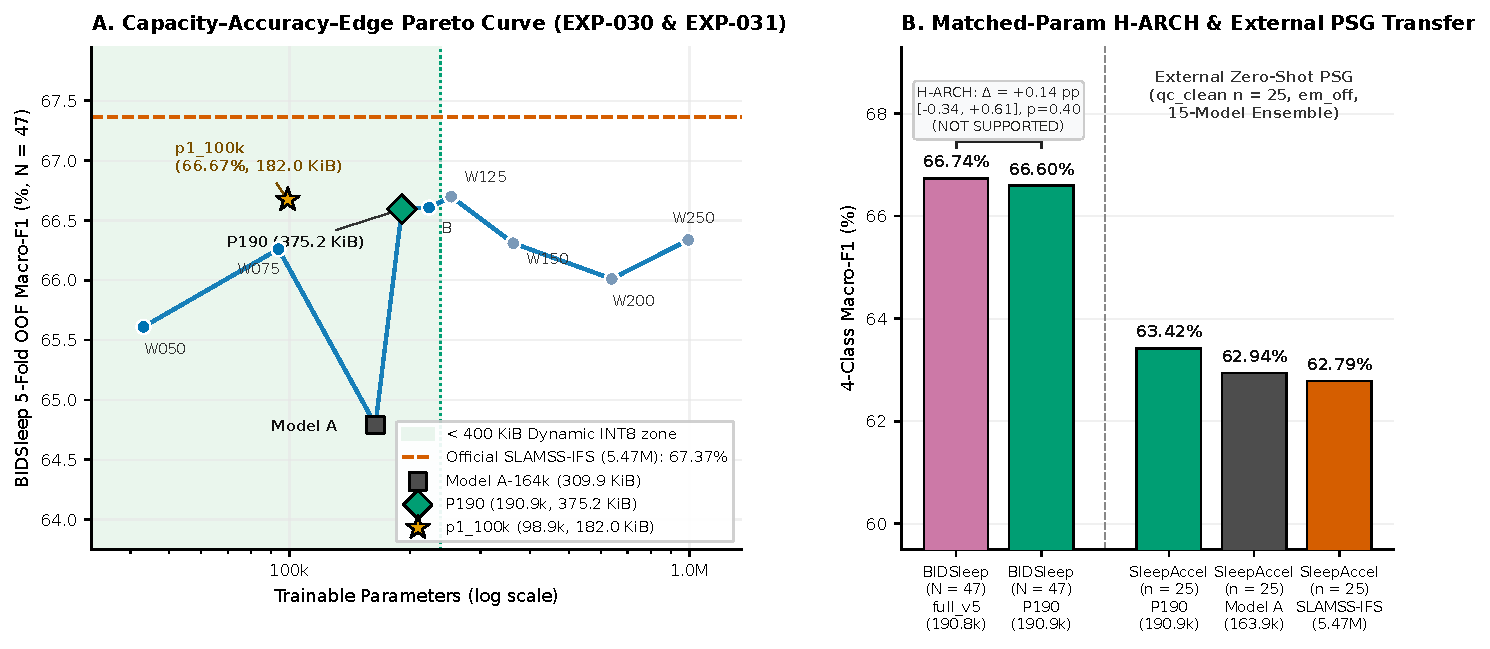
\includegraphics[width=0.92\textwidth]{../figures/manuscript_v2/fig_exp030_exp031_pareto.pdf}
\caption{Capacity scaling, negative architectural ablation, and external PSG transfer. (A) BIDSleep 5-fold OOF Macro-F1 ($N=47$) vs.\ parameters across plain widths (\texttt{W050}--\texttt{W250}) and \texttt{p1\_100k} under $<400$~KiB Dynamic INT8. (B) Parameter-matched \texttt{H-ARCH} ablation (\texttt{full\_v5} vs.\ \texttt{P190}) and SleepAccel zero-shot ensemble Macro-F1 ($n=25$, \texttt{em\_off}).}
\label{fig:pareto}
\end{figure*}

\begin{table}[!t]
\centering
\caption{BIDSleep Capacity Scaling \& Negative Ablation ($N=47$, 100-ep)}
\label{tab:scaling}
\scriptsize
\begin{tabular}{@{}lrrrrr@{}}
\toprule
Model & Params & INT8 (KiB)$^*$ & 4T INT8 (ms)$^\dagger$ & Macro-F1 ($\pm$ SD) & $\Delta$ vs.\ SLAMSS \\
\midrule
\texttt{W050} & 43,108 & 81.00 & --- & $65.61\% \pm 7.48\%$ & $-1.76$~pp \\
\texttt{W075} & 93,796 & 176.96 & --- & $66.26\% \pm 7.10\%$ & $-1.11$~pp \\
\textbf{\texttt{p1\_100k}} & \textbf{98,940} & \textbf{182.00} & \textbf{41.02} & \textbf{$66.67\% \pm 7.57\%$} & \textbf{$-$0.69~pp} \\
\texttt{Model A} (frozen) & 163,940 & 309.54 & --- & $64.79\% \pm 7.45\%$ & $-2.58$~pp \\
\textbf{\texttt{W100} (retrained)} & \textbf{163,940} & \textbf{309.54} & \textbf{43.38} & \textbf{$66.68\% \pm 7.11\%$} & \textbf{$-$0.69~pp} \\
\textbf{\texttt{P190}} & \textbf{190,940} & \textbf{375.16} & \textbf{46.46} & \textbf{$66.60\% \pm 6.85\%$} & \textbf{$-$0.77~pp} \\
\texttt{full\_v5} (Neg.\ Abl.) & 190,788 & 360.50 & 31.53 & $66.74\% \pm 6.81\%$ & $-0.63$~pp \\
\texttt{B} ($w=1.17$) & 223,268 & 368.04 & --- & $66.61\% \pm 7.06\%$ & $-0.76$~pp \\
\texttt{W125} & 253,540 & 479.86 & --- & $66.70\% \pm 6.80\%$ & $-0.67$~pp \\
\texttt{W250} & 993,380 & 1884.63 & --- & $66.34\% \pm 7.05\%$ & $-1.03$~pp \\
\texttt{SLAMSS-IFS} & 5,465,768 & --- & 3186.52 & $67.37\% \pm 6.73\%$ & 0.00~pp \\
\bottomrule
\end{tabular}
\par\vspace{0.2em}\raggedright\scriptsize $^*$Dynamic INT8 serialized weight payload (weights only). $^\dagger$Interleaved round-robin 4T INT8 median latency ($L=1200$, $B=1$, all INT8 CVs $\le 5\%$).
\end{table}

\begin{table}[!t]
\centering
\caption{500-Epoch Convergence Audit on Compact Widths ($N=47$)}
\label{tab:conv500}
\scriptsize
\begin{tabular}{@{}lrrrr@{}}
\toprule
Arm (Params) & 500-ep F1 & $\Delta_{\text{500-100}}$ [95\% CI] & $p_{\text{Holm}}$ (2s) & Ep Mean [Range] \\
\midrule
\texttt{W050\_500ep} (43,108) & 66.24\% & $+0.63$ [$+0.09, +1.09$] & $2.78\times 10^{-3}$ & 184.2 [113, 301] \\
\texttt{W075\_500ep} (93,796) & 66.40\% & $+0.14$ [$-0.15, +0.44$] & $0.5904$ & 130.3 [78, 211] \\
\texttt{p1\_100k\_500ep} (98,940) & 66.68\% & $+0.01$ [$-0.17, +0.18$] & $1.0000$ & 118.9 [81, 154] \\
\texttt{W100\_500ep} (163,940) & 66.70\% & $+0.02$ [$-0.11, +0.15$] & $1.0000$ & 112.2 [65, 141] \\
\bottomrule
\end{tabular}
\end{table}

\subsection{Edge Profile and Quantization}
Table~\ref{tab:edge} reports serialized weight payloads (explicitly \textbf{weights only}), compute (MMACs: 456.1--984.2 vs.\ 40,773.2), and interleaved round-robin CPU latency (\texttt{L=1200}, \texttt{B=1}) on an \texttt{AMD Ryzen 7 7700 8-Core Processor}. We explicitly caveat that these timings reflect a desktop CPU (not an embedded smartwatch SoC) and that bidirectional GRU inference requires full-night $L=1200$ activation buffering (process peak RSS: 800.59~MiB 1T / 799.33~MiB 4T). Dynamic INT8 preserved Macro-F1 within $\pm 0.02$~pp of FP32 (\texttt{p1\_100k}: $-0.0134$~pp, $p=0.4656$; \texttt{W100}: $+0.0011$~pp, $p=0.7892$).

\begin{table*}[!t]
\centering
\caption{Edge Compute, Serialized Weight Payload (Weights Only), and Interleaved CPU Latency ($L=1200$, $B=1$)}
\label{tab:edge}
\scriptsize
\begin{tabular}{@{}lrrrrrrr@{}}
\toprule
Model & FP32 Payload & INT8 (Weights Only) & MMACs & 1T INT8 (ms) & 4T INT8 (ms) & 4T FP32 (ms) & INT8--FP32 $\Delta$ (pp) \\
\midrule
\texttt{p1\_100k} & 386.48~KiB & 182.00~KiB & 456.1 & 47.07 & 41.02 & 40.33 (CV 4.83\%) & $-0.0134$ ($p=0.4656$) \\
\texttt{W100} / \texttt{Model A} & 640.39~KiB & 309.54~KiB & 794.1 & 53.63 & 43.38 & --- (CV $>5\%$) & $+0.0011$ ($p=0.7892$) \\
\texttt{full\_v5} & 745.27~KiB & 360.50~KiB & 847.7 & 43.73 & 31.53 & --- (CV $>5\%$) & $-0.0113$ ($p=0.9041$) \\
\texttt{P190} & 745.86~KiB & 375.16~KiB & 984.2 & 59.41 & 46.46 & --- (CV $>5\%$) & $+0.0244$ ($p=0.0836$) \\
\texttt{SLAMSS-IFS} & 20.85~MiB & --- & 40,773.2 & 3292.75 & 3186.52 & 3261.39 (CV 3.21\%) & --- \\
\bottomrule
\end{tabular}
\end{table*}

\subsection{Multi-Night Personalization ($N=46$; \texttt{W100} Primary \& Legacy \texttt{Model~A})}
On recipe-consistent \texttt{W100} ($N=46$, Table~\ref{tab:pers}, Fig.~\ref{fig:forest}), typical participants gained about $+0.6$ to $+0.75$~pp (\texttt{W100} median $+0.75$~pp, 95\% CI $[+0.11, +1.28]$, 30 wins to 16 losses), which is statistically detectable ($p_{\text{Holm}}=0.0263$) but below the preregistered $+1.50$~pp practical threshold (\textbf{NOT SUPPORTED practically}); the mean CI ($+0.58$~pp, 95\% CI $[-0.06, +1.22]$) includes zero because a few participants lost more, and every fold selected the boundary configuration (\texttt{lr = 3e-5}, head + last GRU), consistent with a small effect. Donor specificity \texttt{S-SPEC} (\texttt{FT-2 - FT-other-2}) was $+1.45$~pp ($[+0.89, +2.02]$, $p_{\text{Holm}}=2.47\times 10^{-5}$, \textbf{INCONCLUSIVE}), driven in part by $-0.87$~pp donor harm relative to \texttt{ZS}. Calibration depth scaling on $E_4$ ($N=33$, $k=1$--4, Fig.~\ref{fig:depth}) was null (Page's $L=835.0$, $z=+0.573$, raw two-sided $p=0.5667$, raw one-sided $p=0.2834$), and descriptive \texttt{GATE\_tau} ($\tau=1\%\text{--}5\%$) failed to prevent worst-case losses ($\text{min }\Delta = -5.18$~pp on \texttt{W100}; no gating benefit claimed). By contrast, legacy frozen \texttt{Model~A} (\textbf{older recipe}) yielded $+1.01$~pp (\texttt{+1.0054~pp}, 95\% CI $[-0.17, +1.99]$, 34/46 wins, locked one-sided $p=0.00131$, two-sided $p=0.00261$).

\begin{table}[!t]
\centering
\caption{Two-Night Personalization (\texttt{FT-2 - ZS} \& \texttt{S-SPEC}, $N=46$)}
\label{tab:pers}
\scriptsize
\begin{tabular}{@{}lrrrrr@{}}
\toprule
Backbone & Mean $\Delta$ & Median $\Delta$ & 95\% Mean CI & W/L/T & \texttt{FT-2 - other} \\
\midrule
\textbf{\texttt{W100}} (Primary) & $+0.58$ & $+0.75$ & $[-0.06, +1.22]$ & 30/16/0 & $+1.45$ [$+0.89, +2.02$] \\
\texttt{p1\_100k} & $+0.51$ & $+0.70$ & $[+0.03, +0.95]$ & 31/15/0 & $+1.09$ [$+0.62, +1.56$] \\
\texttt{P190} & $-0.02$ & $+0.69$ & $[-1.09, +0.85]$ & 31/15/0 & $+0.64$ [$-0.29, +1.47$] \\
\texttt{full\_v5} & $+0.45$ & $+1.03$ & $[-0.57, +1.41]$ & 28/18/0 & $+1.27$ [$+0.41, +2.06$] \\
\texttt{Model A} (older) & $+1.01$ & $+1.55$ & $[-0.17, +1.99]$ & 34/12/0 & $+2.73$ [$+1.05, +4.38$] \\
\bottomrule
\end{tabular}
\end{table}

\begin{figure}[!t]
\centering
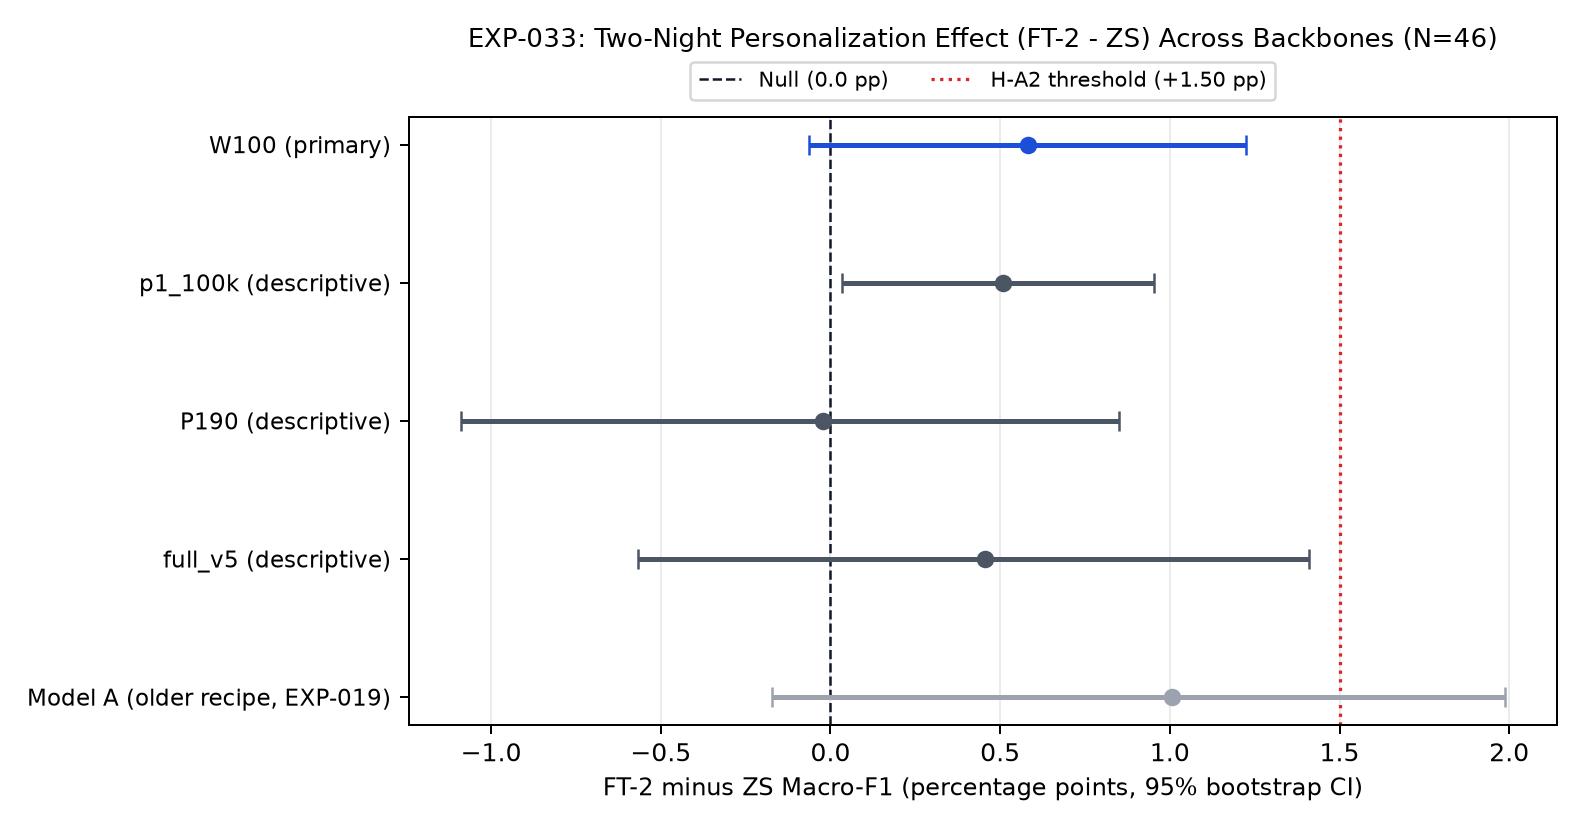
\includegraphics[width=\linewidth]{../figures/manuscript_v2/backbone_forest_plot.png}
\caption{Two-night personalization (\texttt{FT-2 - ZS}, $N=46$) across recipe-consistent backbones and legacy frozen \texttt{Model~A} (older recipe).}
\label{fig:forest}
\end{figure}

\begin{figure}[!t]
\centering
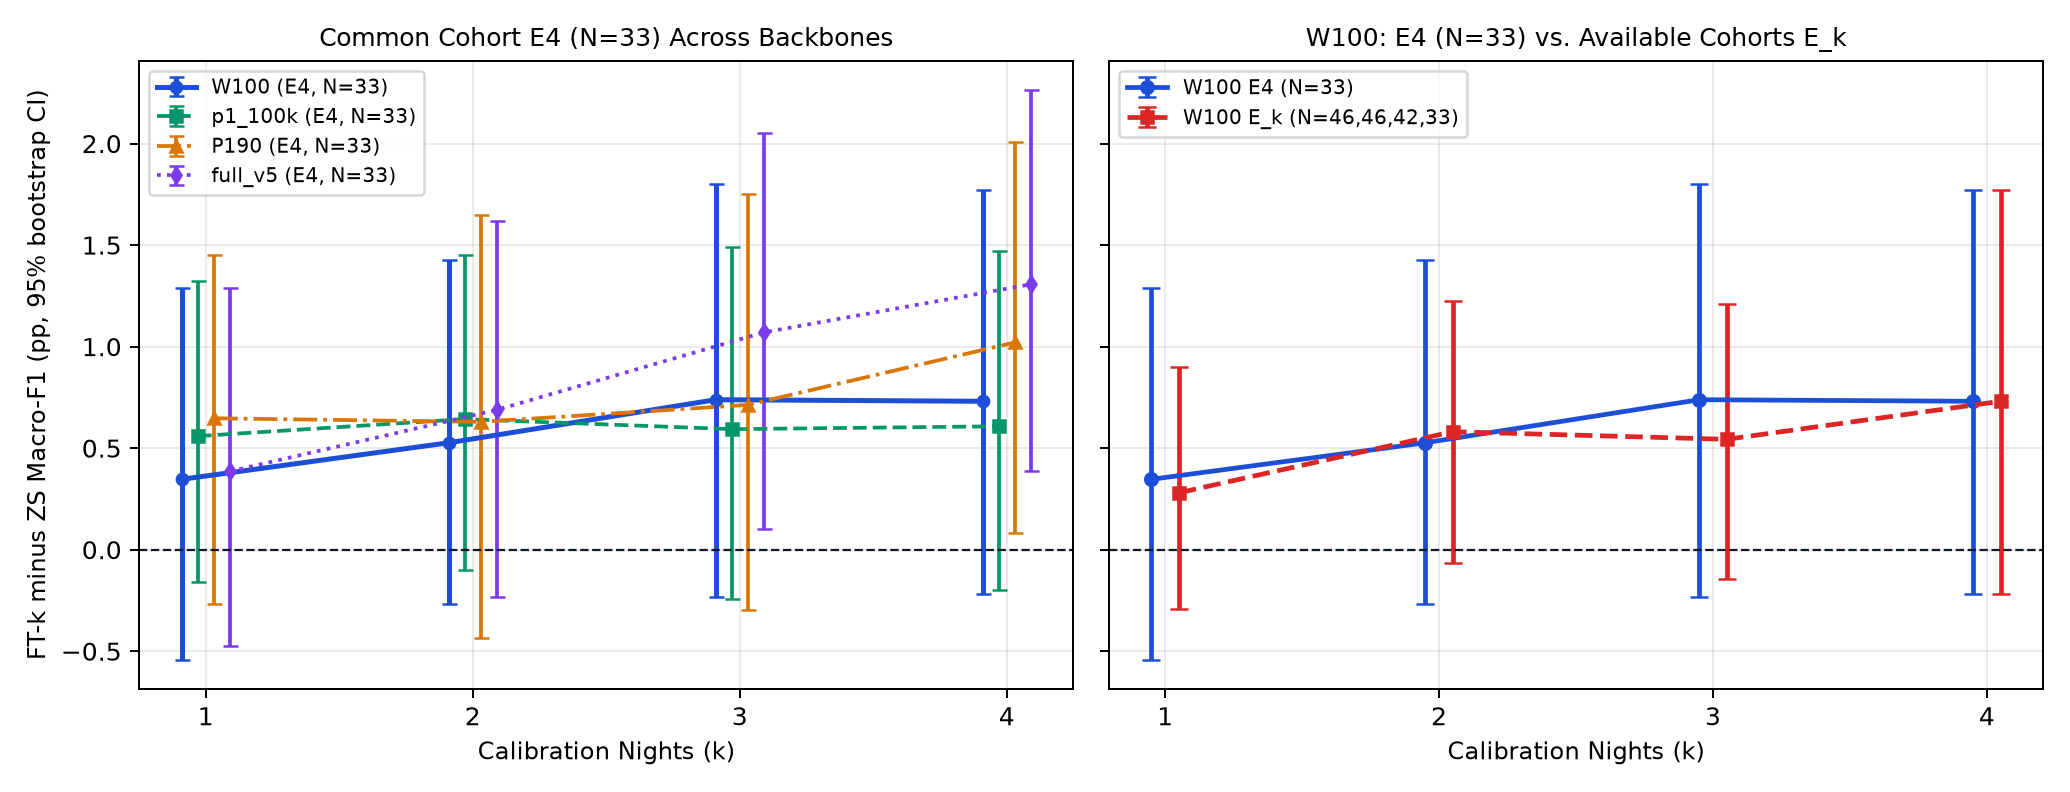
\includegraphics[width=\linewidth]{../figures/manuscript_v2/depth_curve.png}
\caption{Calibration-depth curve ($k=1$--4 nights) on \texttt{W100} ($E_4$ $N=33$, null Page's $L=835.0$, $p=0.5667$) with 95\% bootstrap CI error bars.}
\label{fig:depth}
\end{figure}

\subsection{Zero-Shot External SleepAccel PSG Validation ($n=25$ / $N=31$)}
Under strictly zero-shot \texttt{em\_off} evaluation (Table~\ref{tab:sleepaccel}), \texttt{W100} achieved 61.23\% single-model ($+0.71$~pp vs.\ \texttt{Model~A} 60.51\%, raw $p=0.1014$; $+0.14$~pp $[-1.28, +1.56]$ vs.\ SLAMSS-IFS 61.08\%, raw $p=0.9578$) and 62.93\% ensemble on $n=25$ (61.58\% / 63.43\% on $N=31$), representing \textbf{no statistically significant difference (a difference is not excluded given the 2.36~pp 80\% MDE)}. Reconciled single/ensemble Macro-F1 across \texttt{p1\_100k} (60.88\%/62.51\%), \texttt{P190} (61.52\%/63.42\%), and \texttt{full\_v5} (61.78\%/63.51\%) confirmed consistent external transfer, whereas unsupervised EM prior correction (\texttt{em\_on}) degraded Macro-F1 ($63.51\% \rightarrow 61.30\%$). In Bland--Altman agreement ($n=25$, descriptive only, \textbf{no clinical-agreement claim}), \texttt{W100} overestimated REM\% ($+12.23\%$) and Deep\% ($+7.10\%$) while underestimating WASO ($-14.48$~min; TST $+12.12$~min, SOL $+3.24$~min, SE $+2.67\%$), reflecting Dreem~2 vs.\ in-lab PSG scoring shift.

\begin{table}[!t]
\centering
\caption{Reconciled Zero-Shot SleepAccel Macro-F1 (\texttt{em\_off}, \%)}
\label{tab:sleepaccel}
\scriptsize
\begin{tabular}{@{}lrrrr@{}}
\toprule
Model & \texttt{qc\_clean} 1-Mod & \texttt{qc\_clean} Ens & \texttt{all} 1-Mod & \texttt{all} Ens \\
\midrule
\texttt{Model A} (older) & 60.51 & 62.94 & 60.65 & 62.94 \\
\texttt{p1\_100k} & 60.88 & 62.51 & 61.10 & 62.51 \\
\texttt{W100} & 61.23 & 62.93 & 61.58 & 63.43 \\
\texttt{P190} & 61.52 & 63.42 & 61.77 & 63.94 \\
\texttt{full\_v5} & 61.78 & 63.51 & 62.30 & 64.21 \\
\texttt{SLAMSS-IFS} & 61.08 & 62.79 & 62.27 & 64.14 \\
\bottomrule
\end{tabular}
\par\vspace{0.2em}\raggedright\scriptsize Note: \texttt{Model A} (\texttt{62.9385\%} vs.\ \texttt{62.9366\%}) and \texttt{p1\_100k} (\texttt{62.5057\%} vs.\ \texttt{62.5105\%}) ensemble values are independently computed and coincide at 2-decimal rounding. On \texttt{qc\_clean} single-model \texttt{Model A} vs.\ \texttt{SLAMSS-IFS}, accuracy (10/15 wins) and Wake F1 (15/10 wins) share identical Wilcoxon $W=106.0$ ($p=0.1336$) due to an exact mirrored signed-rank sum pattern ($W^+=106.0$, $W^-=219.0$ vs.\ $W^+=219.0$, $W^-=106.0$).
\end{table}

\begin{table}[!t]
\centering
\caption{External SleepAccel Bland--Altman Agreement ($n=25$, \texttt{em\_off}; Descriptive Only, No Clinical-Agreement Claim)}
\label{tab:sleepaccel_ba}
\scriptsize
\begin{tabular}{@{}lrrrr@{}}
\toprule
Metric & \texttt{W100} (1-Mod) & \texttt{P190} (Ens) & \texttt{Model A} (Ens) & \texttt{SLAMSS-IFS} (Ens) \\
\midrule
TST (min) & $+12.12$ & $+10.14$ & $+12.22$ & $+15.72$ \\
SOL (min) & $+3.24$ & $+4.48$ & $+2.44$ & $+0.38$ \\
WASO (min) & $-14.48$ & $-13.80$ & $-13.82$ & $-15.16$ \\
SE (\%) & $+2.67$ & $+2.24$ & $+2.71$ & $+3.49$ \\
Deep\% TST & $+7.10$ & $+7.24$ & $+10.23$ & $+8.84$ \\
REM\% TST & $+12.23$ & $+10.98$ & $+9.35$ & $+6.87$ \\
\bottomrule
\end{tabular}
\end{table}

\begin{figure}[!t]
\centering
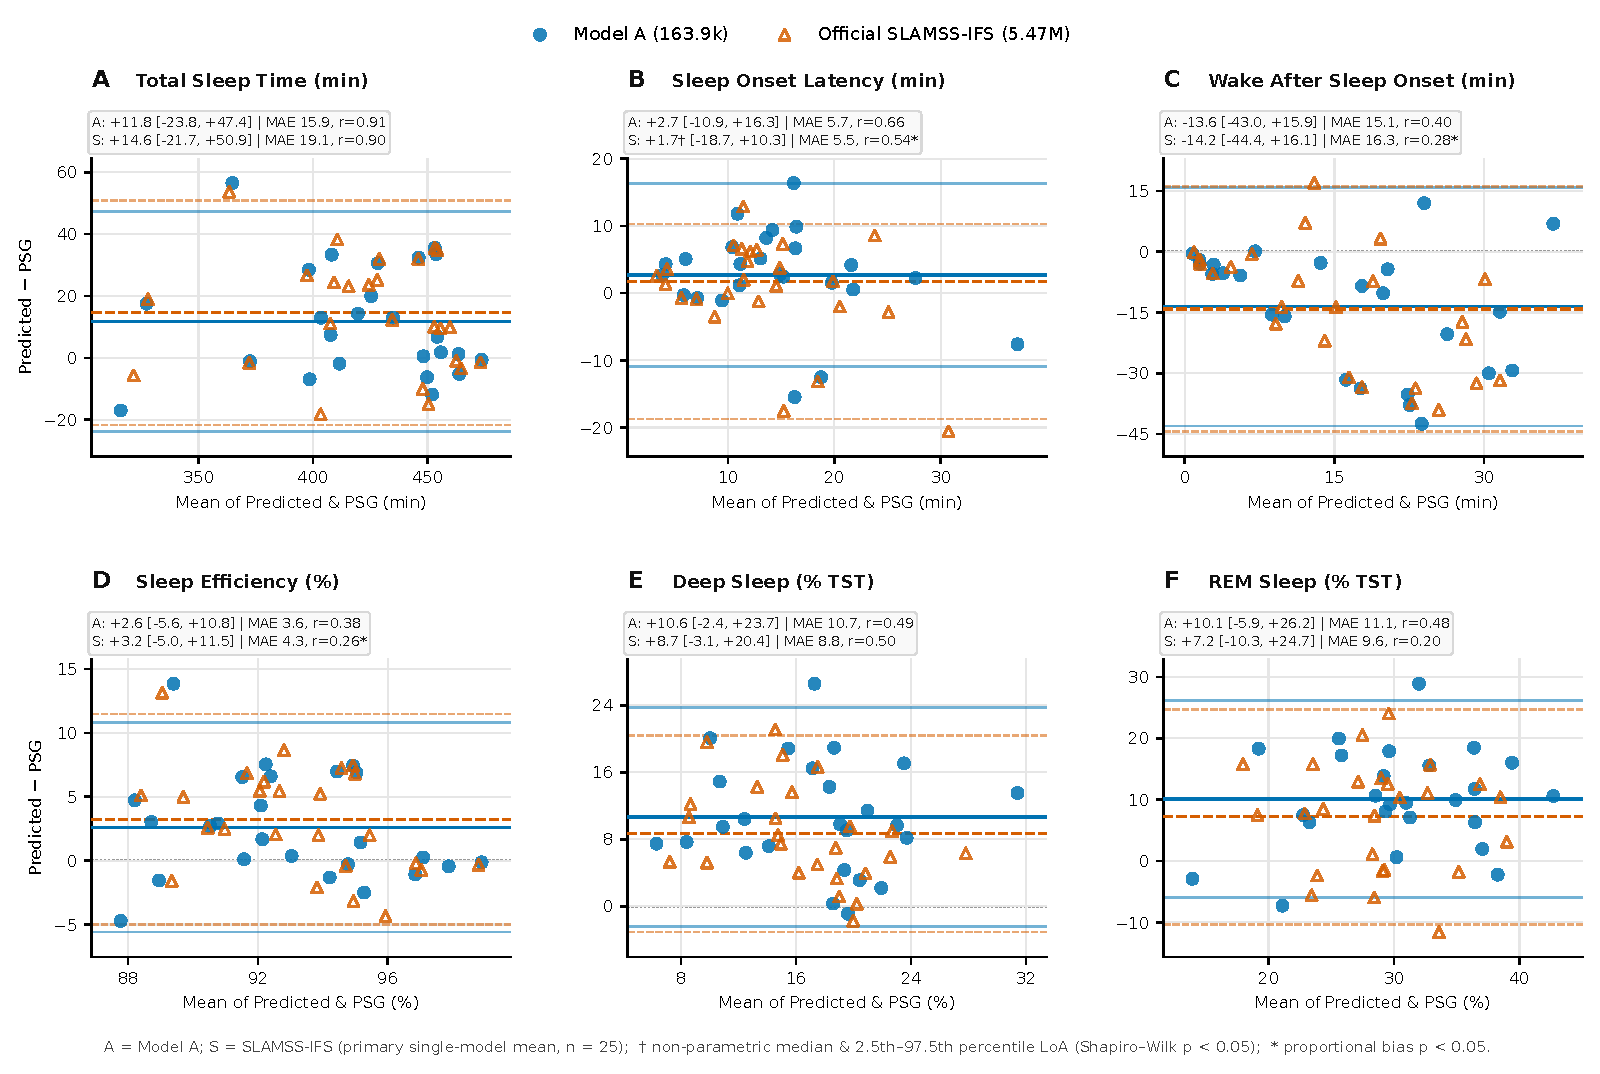
\includegraphics[width=\linewidth]{../figures/manuscript_v2/Figure4_External_PSG_Bland_Altman.pdf}
\caption{External SleepAccel Bland--Altman agreement ($n=25$, descriptive only, no clinical-agreement claim) showing systematic Deep\% and REM\% overestimation.}
\label{fig:ba}
\end{figure}

\begin{figure}[!t]
\centering
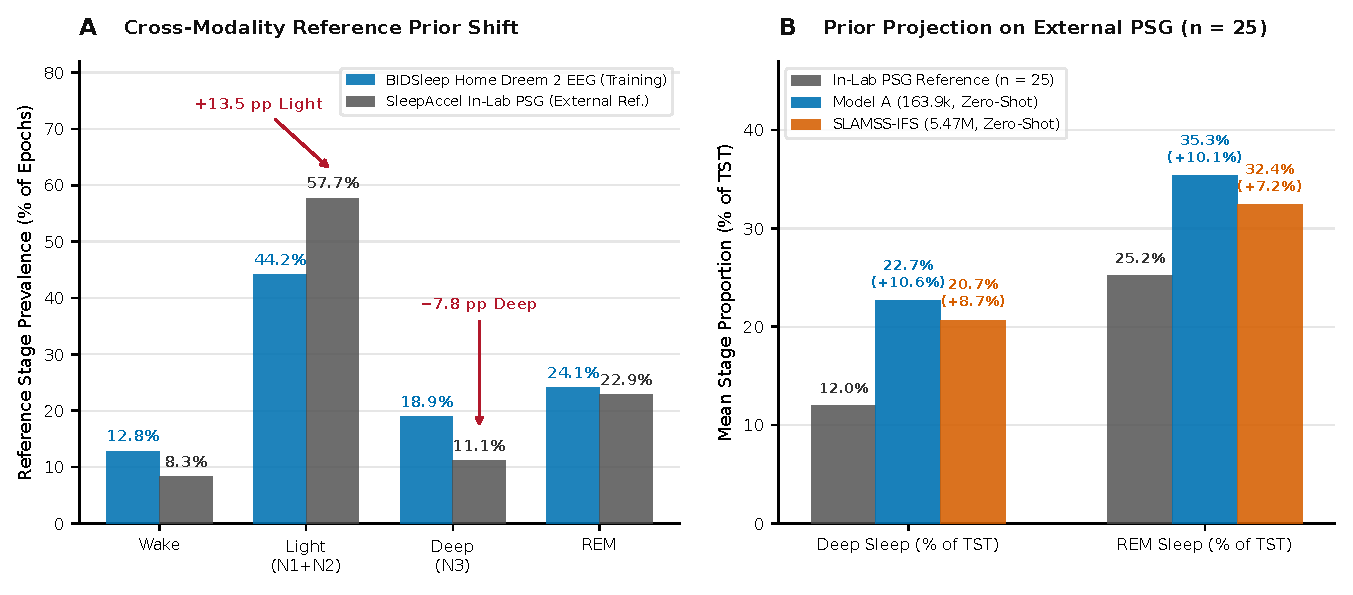
\includegraphics[width=\linewidth]{../figures/manuscript_v2/Figure5_Label_Prior_Shift_Diagnosis.pdf}
\caption{Cross-modality reference stage-prior shift between home Dreem~2 EEG (BIDSleep) and in-lab PSG (SleepAccel).}
\label{fig:prior}
\end{figure}

\section{Discussion and Conclusion}
Our pre-registered audit establishes that training-recipe consistency---not architectural complexity---drives the performance of compact smartwatch sleep-staging models. Unifying the recipe raised 164k-parameter \texttt{Model~A} by $+1.89$~pp to 66.68\% (\texttt{W100}), and extending training to 500 epochs confirmed that \texttt{p1\_100k} (98,940 params, 182.00~KiB INT8 weights, 41.02~ms) and \texttt{W100} were already converged at 100 epochs, while FiLM + 2-scale pooling (\texttt{full\_v5}) offered no benefit over parameter-matched \texttt{P190}. Under rate-limited ($\sim$0.20~Hz) IHR + ACC, two-night personalization produced small, practically sub-threshold gains on \texttt{W100} (median $+0.75$~pp, 30W/16L) and null depth scaling, and zero-shot clinical PSG evaluation showed no statistically significant difference against 5.47M SLAMSS-IFS (with systematic Deep\%/REM\% overestimation precluding clinical-agreement claims). All findings are scoped to healthy adults and offline $L=1200$ buffering; prospective validation in clinical (DREAMT v2.2.0) and multi-night cohorts (Simons Sleep Project) is warranted.

\begin{thebibliography}{15}
\bibitem{berry2020aasm} R.~B. Berry et al., \textit{The AASM Manual for the Scoring of Sleep and Associated Events}, v2.6. Darien, IL: AASM, 2020.
\bibitem{song2026bidsleep} T.~A. Song et al., ``AI-driven sleep staging using instantaneous heart rate and accelerometry: insights from an Apple Watch study,'' \textit{IEEE Trans. Biomed. Eng.}, vol.~73, no.~4, pp.~1596--1608, 2026, doi:10.1109/TBME.2025.3612158.
\bibitem{bidsleep_data} T.~Song, Y.~Zhang, Z.~Zhou, and J.~Dutta, ``A Multi-Night Instantaneous Heart Rate and Accelerometry Dataset with EEG Sleep Stage Labels (version 1.0.1),'' \textit{PhysioNet}, 2026, doi:10.13026/rees-1092.
\bibitem{walch2019sleepaccel} O.~Walch, Y.~Huang, D.~Forger, and C.~Goldstein, ``Sleep stage prediction with raw acceleration and photoplethysmography heart rate data derived from a consumer wearable device,'' \textit{Sleep}, vol.~42, no.~12, p.~zsz180, 2019, doi:10.1093/sleep/zsz180.
\bibitem{walch2019sleepaccel_data} O.~Walch, ``Motion and heart rate from a wrist-worn wearable and labeled sleep from polysomnography (version 1.0.0),'' \textit{PhysioNet}, 2019, doi:10.13026/hmhs-py35.
\bibitem{vanderaar2025ppg} J.~F. van der Aar et al., ``Learning individual autonomic representations of sleep stages to improve photoplethysmography based sleep monitoring,'' \textit{Physiol. Meas.}, vol.~46, no.~9, p.~095012, 2025.
\bibitem{beattie2017ppg} Z.~Beattie et al., ``Estimation of sleep stages in a healthy adult population from optical plethysmography and accelerometer signals,'' \textit{Physiol. Meas.}, vol.~38, no.~11, pp.~1968--1979, 2017.
\bibitem{brookshire2024leakage} G.~Brookshire et al., ``Data leakage in deep learning studies of translational EEG,'' \textit{Front. Neurosci.}, vol.~18, p.~1373515, 2024.
\bibitem{bland1999agreement} J.~M. Bland and D.~G. Altman, ``Measuring agreement in method comparison studies,'' \textit{Stat. Methods Med. Res.}, vol.~8, no.~2, pp.~135--160, 1999.
\bibitem{collins2024tripod} G.~S. Collins et al., ``TRIPOD+AI statement: updated guidance for reporting clinical prediction models that use regression or machine learning methods,'' \textit{BMJ}, vol.~385, p.~e078378, 2024.
\bibitem{phan2023lseqsleepnet} H.~Phan, K.~P. Lorenzen, E.~Heremans, O.~Y. Ch\'en, M.~C. Tran, P.~Koch, A.~Mertins, M.~Baumert, K.~B. Mikkelsen, and M.~De Vos, ``L-SeqSleepNet: Whole-cycle long sequence modelling for automatic sleep staging,'' \textit{IEEE J. Biomed. Health Inform.}, vol.~27, no.~10, pp.~4748--4757, 2023, doi:10.1109/JBHI.2023.3303197.
\bibitem{heremans2022adaptation} E.~R.~M. Heremans, H.~Phan, P.~Borz\'ee, B.~Buyse, D.~Testelmans, and M.~De Vos, ``From unsupervised to semi-supervised adversarial domain adaptation in electroencephalography-based sleep staging,'' \textit{J. Neural Eng.}, vol.~19, no.~3, 2022, doi:10.1088/1741-2552/ac6ca8.
\bibitem{heremans2022feature} E.~R.~M. Heremans, H.~Phan, A.~H. Ansari, P.~Borz\'ee, B.~Buyse, D.~Testelmans, and M.~De Vos, ``Feature matching as improved transfer learning technique for wearable EEG,'' \textit{Biomed. Signal Process. Control}, vol.~78, p.~104009, 2022.
\bibitem{page1963ordered} E.~B. Page, ``Ordered hypotheses for multiple treatments: a significance test for linear ranks,'' \textit{J. Am. Stat. Assoc.}, vol.~58, no.~301, pp.~216--230, 1963.
\bibitem{oldham1962note} P.~D. Oldham, ``A note on the analysis of repeated measurements of the same subjects,'' \textit{J. Chronic Dis.}, vol.~15, no.~10, pp.~969--977, 1962.
\end{thebibliography}

\end{document}
